\documentclass[11pt,oneside]{book}
\usepackage[margin=1.2in]{geometry}
\usepackage[toc,page]{appendix}
\usepackage{graphicx}
% \usepackage{natbib}
\usepackage{lipsum}
% \usepackage{caption}
\usepackage{etoolbox}
\usepackage[hidelinks]{hyperref}
\usepackage{tikz}
\usepackage{listings}
\usepackage{verbatim}

\usetikzlibrary{shapes.geometric, arrows}

\usepackage[style=ieee]{biblatex}

\usepackage{xcolor}
 
\definecolor{codegreen}{rgb}{0,0.6,0}
\definecolor{codegray}{rgb}{0.5,0.5,0.5}
\definecolor{codepurple}{rgb}{0.58,0,0.82}
\definecolor{backcolour}{rgb}{0.95,0.95,0.92}
 
\lstdefinestyle{mystyle}{
    backgroundcolor=\color{backcolour},   
    commentstyle=\color{codegreen},
    keywordstyle=\color{magenta},
    numberstyle=\tiny\color{codegray},
    stringstyle=\color{codepurple},
    basicstyle=\ttfamily\footnotesize,
    breakatwhitespace=false,         
    breaklines=true,                 
    captionpos=b,                    
    keepspaces=true,                 
    numbers=left,                    
    numbersep=5pt,                  
    showspaces=false,                
    showstringspaces=false,
    showtabs=false,                  
    tabsize=2
}
 
\lstset{style=mystyle}
 
\bibliography{mybibliography.bib} 
\makeatletter
\patchcmd{\@makechapterhead}% <cmd>
  {\@chapapp\space\thechapter\par\nobreak\vskip 20\p@}% <search>
  {\Huge\thechapter\space}% <replace>
  {}{}% <success><failure>
\makeatother
\begin{document}

\frontmatter

\begin{titlepage}
\begin{center}
{\LARGE \textbf{Assignment 8}}\\[1cm]\LARGE {\textbf{ELP-780 Software Lab}}\\[0.3cm]
{\Large \textbf{Asmita Patil}}\\[0.25cm]
{\Large \textbf{2018EET2560}}\\[0.25cm]
{\Large \textbf{2019-20}}\\[1cm]
{\Large A report presented for the assignment}\\[1cm]
{\Large \textbf{Python and Github }
\hyperlink{https://github.com/eet182560/Assignment_8/}{GitHub Link}}\\[2cm]
\linespread{1}

\includegraphics[width=5cm]{Software_Lab_Template/images/redt.png}\\[2cm]
{\large \textbf{Computer Technology}}\\[0.25cm] % if applicable
\large \textbf{Department of Electrical Engineering}\\[0.25cm] 
\large \textbf{IIT DELHI}\\[0.25cm]
\large \textbf{India}\\[0.3cm]
\textbf{\today}
\end{center}

\end{titlepage}
\tableofcontents
\mainmatter

\chapter{\textbf{Problem Statement-1}}
\section{Problem Statement}
\begin{itemize}
    \item \textbf{Parity Check}
    \item The simplest way of error detection is to append a single bit, called a parity check, to a string of data bits. 
    \item This parity check bit has the value 1 if the number of 1’s in the bit string is even and has the value 0 otherwise, i.e., Odd Parity Check.
    \item \textbf{Bit-Oriented Framing}
    \item Data Link Layer needs to pack bits into frames so that each frame is distinguishable from another. 
    \item Frames can be fixed or variable size. In variable size framing, we define the end of the frame using a bit-oriented approach. 
    \item It uses a special string of bits, called a flag for both idle fills and to indicate the beginning and the ending of frames.
    \item The bit stuffing rule is to insert a 0 after each appearance of 010 in the original data. 
    \item The string 0101 is used as the bit string or flag to indicate the end of the frame.

\end{itemize}

\section{Assumptions}
\begin{itemize}
    \item Compiler for Python and all required libraries are already installed.
    \item User is familiar with all concepts of Python required for assignment.\cite{Reference2}
    \item User have experience with Github and Makefile.\cite{Reference1}
\end{itemize}

\section{Program Structure}

% Define block styles
\tikzstyle{decision} = [diamond, draw, fill=red!30, 
    text width=4.5em, text badly centered, node distance=3cm, inner sep=0pt]
\tikzstyle{block} = [rectangle, draw, fill=blue!20, 
    text width=6em, text centered, rounded corners, minimum height=4em]
\tikzstyle{line} = [draw, -latex']
\tikzstyle{cloud} = [draw, ellipse,fill=red!20, node distance=3cm,
    minimum height=2em]
    
\begin{tikzpicture}[node distance = 2cm, auto]
    % Place nodes
    \node [block] (init) {Start};
    \node [block, below of=init] (identify) {Take binary input string from user};
    \node [decision, below of=identify] (decide1) {Is input valid?};
    \node [block, below of=decide1, node distance=3cm] (evaluate) {Calculate parity using odd parity check};
    \node [block, below of=evaluate, node distance=3cm] (evaluate1) {Display parity data to user};
    \node [block, below of=evaluate1] (evaluate2) {Perform bit stuffing operation};
    \node [block, below of=evaluate2] (evaluate3) {Display Transmitting data to user};

    \node [block, below of=evaluate3, node distance=2cm] (stop) {stop};
    % Draw edges
    \path [line] (init) -- (identify);
    \path [line] (identify) -- (decide1);
    \path [line] (decide1) -- node {yes} (evaluate);
    \path [line] (evaluate) -- (evaluate1);
    \path [line] (evaluate1) -- (evaluate2);
    \path [line] (evaluate2) -- (evaluate3);
    \path [line] (evaluate3) -- (stop);
    \path [line] (decide1.west) to[out=180,in=150] (stop.west);

\end{tikzpicture}


\section{Algorithm and Implementation}
Problem can be solved when execution is done in following steps:
\textit{
\begin{itemize}
    \item Take binary input string from user.
    \item Check the string is valid or not. If not valid exit with error.
    \item Calculate the parity for given string and append it at the end of string.
    \item This parity check bit has the value 1 if the number of 1’s in the bit string is even and has the value 0 otherwise, i.e., Odd Parity Check.
    \item Perform bit stuffing to handle flag properly.
    \item Initialize all variables required for execution and calculation.
    \item Print parity data and transmitting data to the user.
\end{itemize}
}

Implementation is done in python and screen-shots and code snippet is also provided.\\
During the implementation, I have fork and cloned GIT project and performed following git commands.
\begin{itemize}
    \item git add
    \item git commit
    \item git status
    \item git log
\end{itemize}

\section{Input and Output format}
\begin{itemize}
    \item \textbf{Input : }
    \begin{itemize}
        \item Enter binary bit data that has to be transmitted.
        \item \textbf{Sample Input}\\010101110100101

    \end{itemize}

    \item \textbf{Output : }
    \begin{itemize}
        \item Print binary bit data with parity bit.
        \item Print the modified string that is to be transmitted
        \item \textbf{Sample Output}\\Parity bit data : 0101011101001011\\
Transmitting data: 01001011101000100110101
    \end{itemize}
    
\end{itemize}

\section{Test cases}
Following test cases are executed :
\begin{itemize}
    \item Input which gives parity 0 is executed
    \item Input which gives parity 1 is executed\\
Screenshots are attached for the same
\end{itemize}

\section{Difficulties/Issues faced}
\begin{itemize}
    \item Inserting 0 for bit stuffing. Created new list of character to solve this.
\end{itemize}

\section{Screenshots}
Following are the screenshots
\begin{figure}[h]
    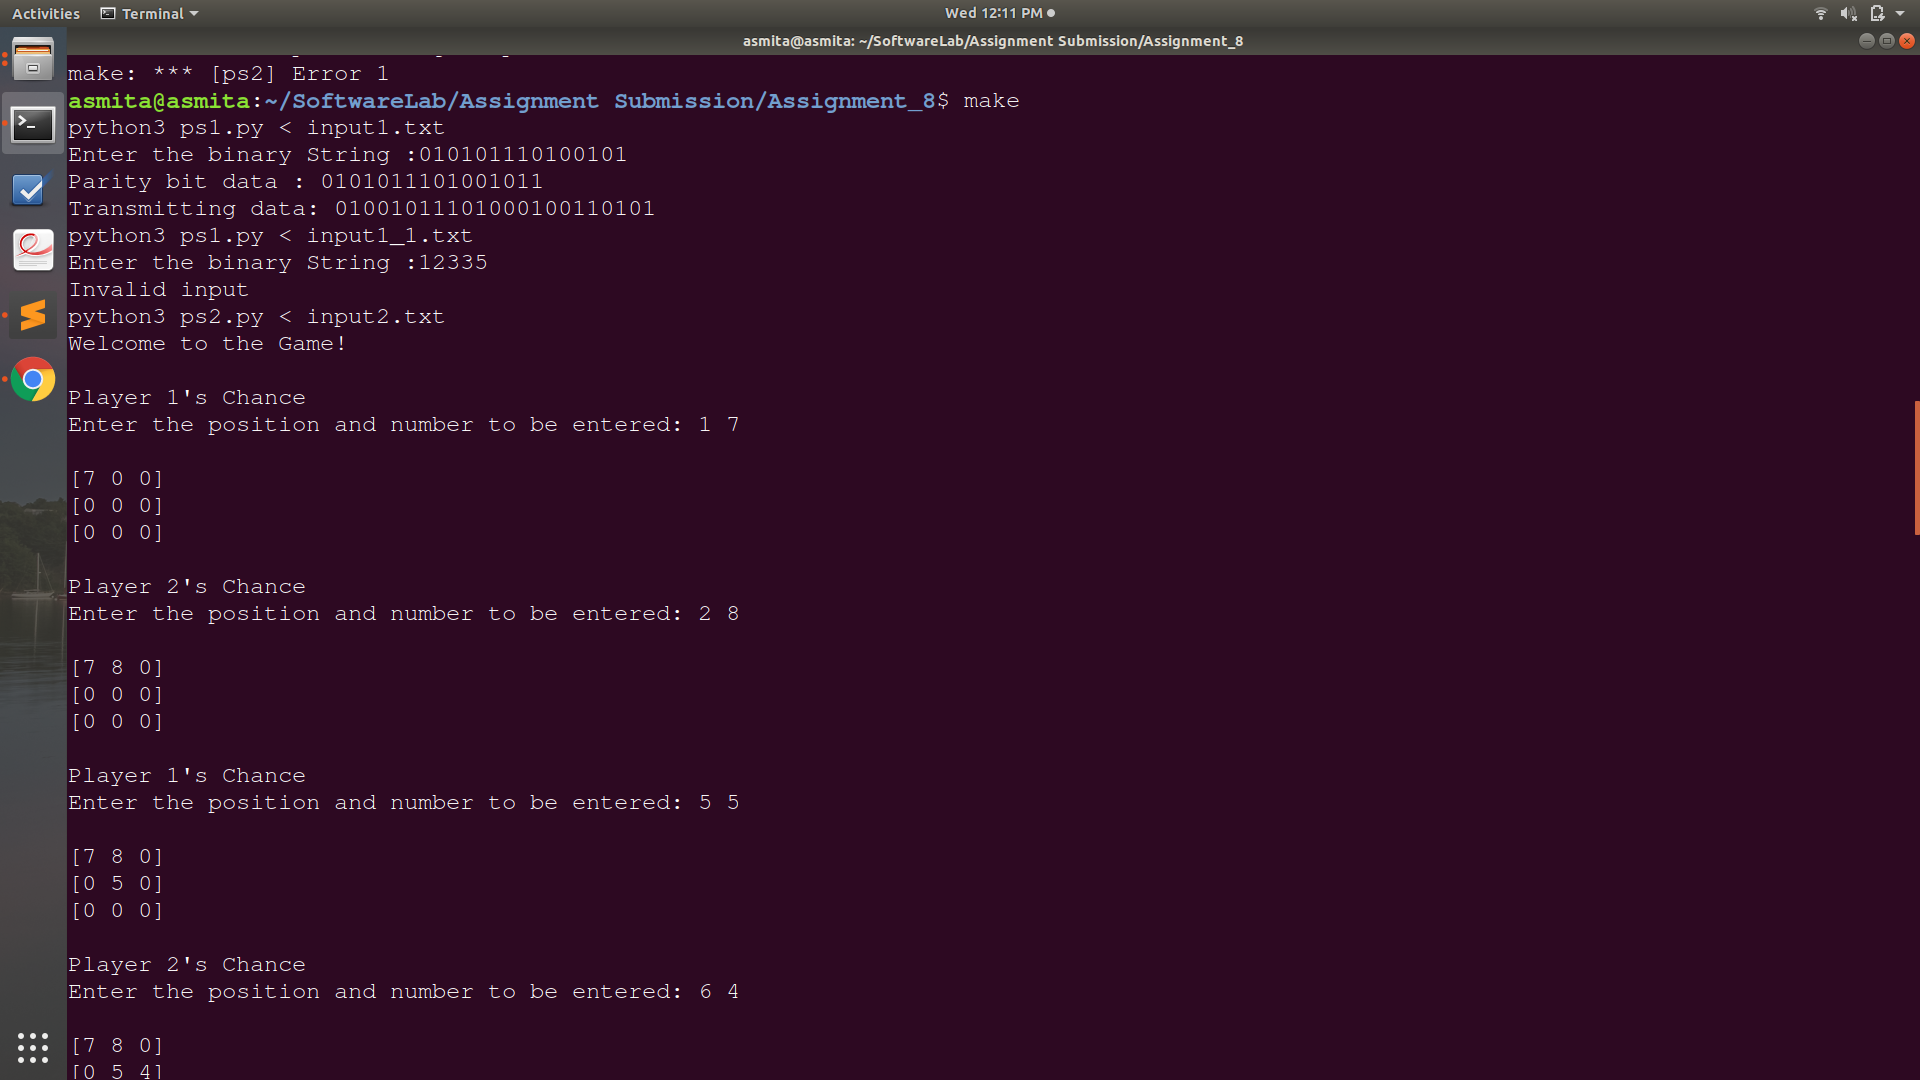
\includegraphics[width=1\textwidth]{Software_Lab_Template/images/makeFileAndPs1.png}
  \caption{Execution of problem statement 1 and Running makefile}
  \label{fig:Problem statement 1 and Makefile}
\end{figure}
\begin{figure}[h]
    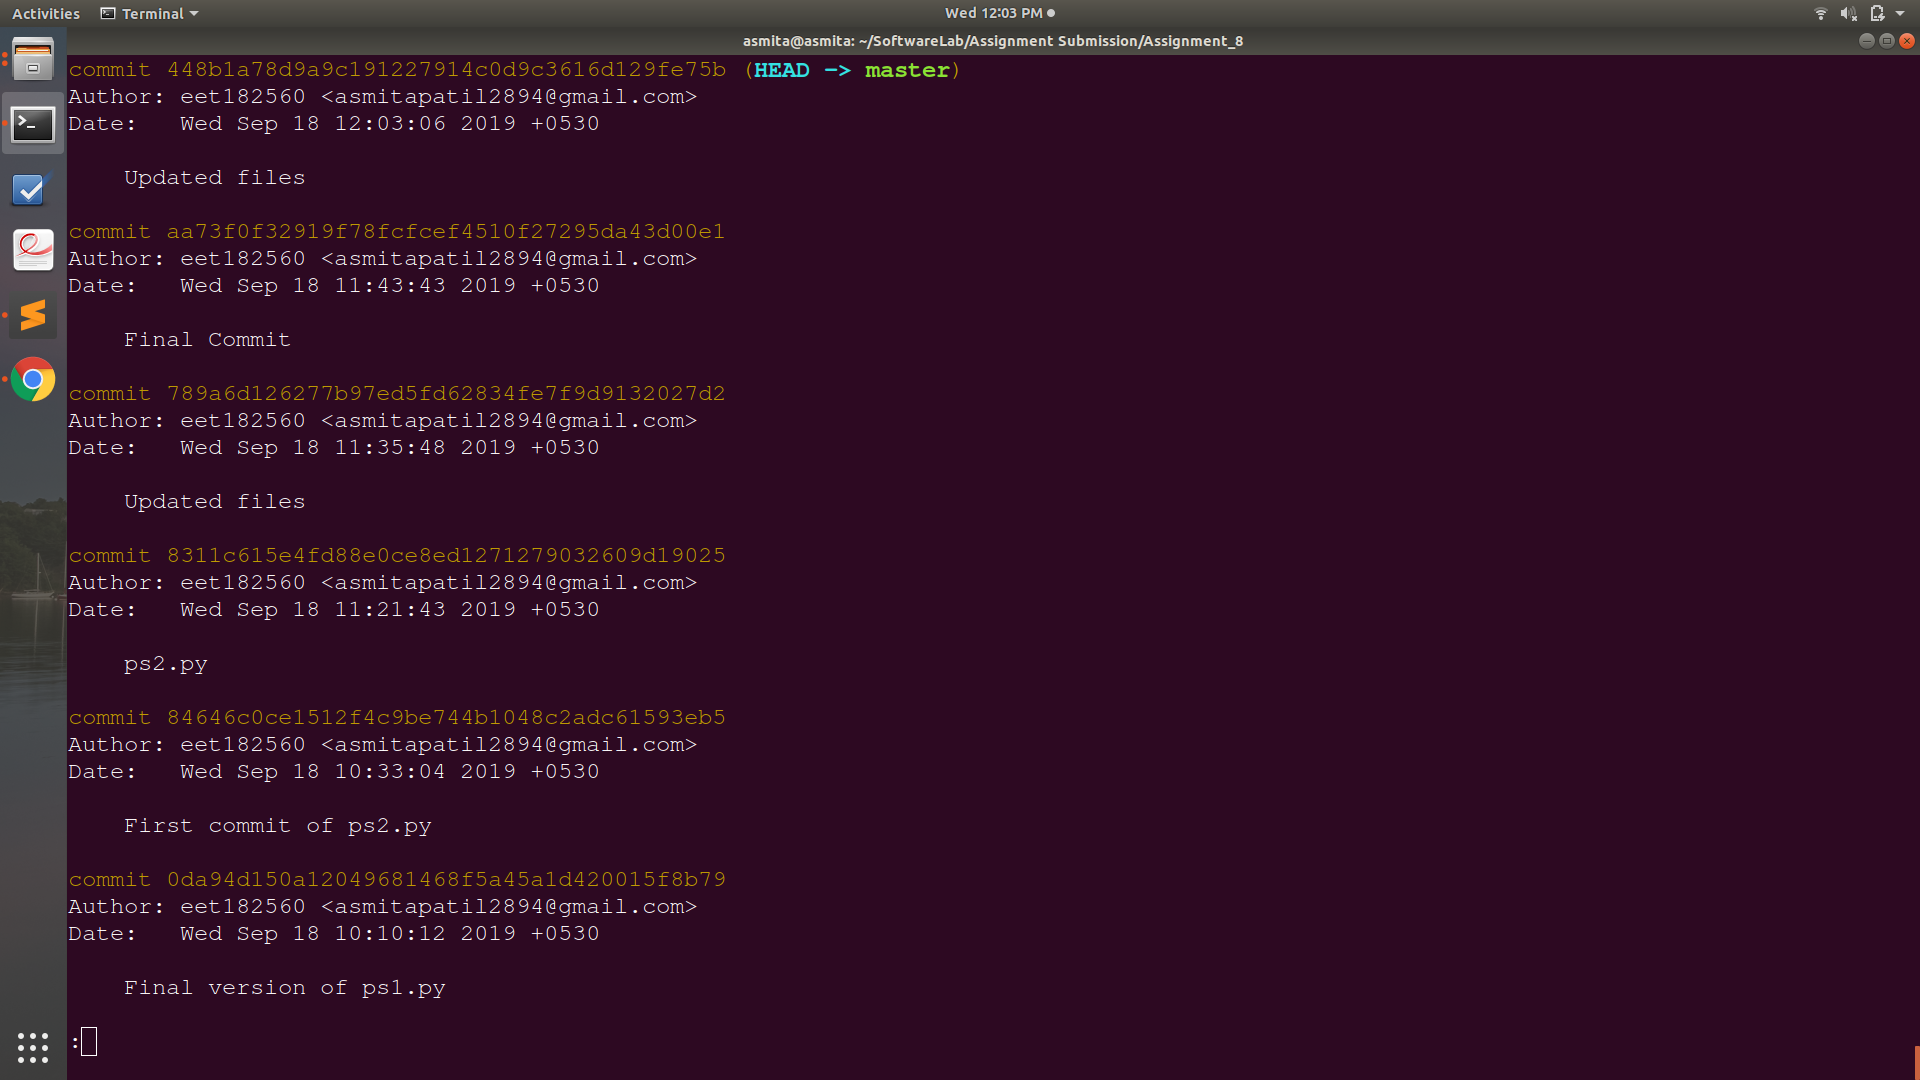
\includegraphics[width=1\textwidth]{Software_Lab_Template/images/git1.png}
  \caption{Execution of Git Command}
  \label{fig:Execution of Git Command}
\end{figure}
\begin{figure}[h]
    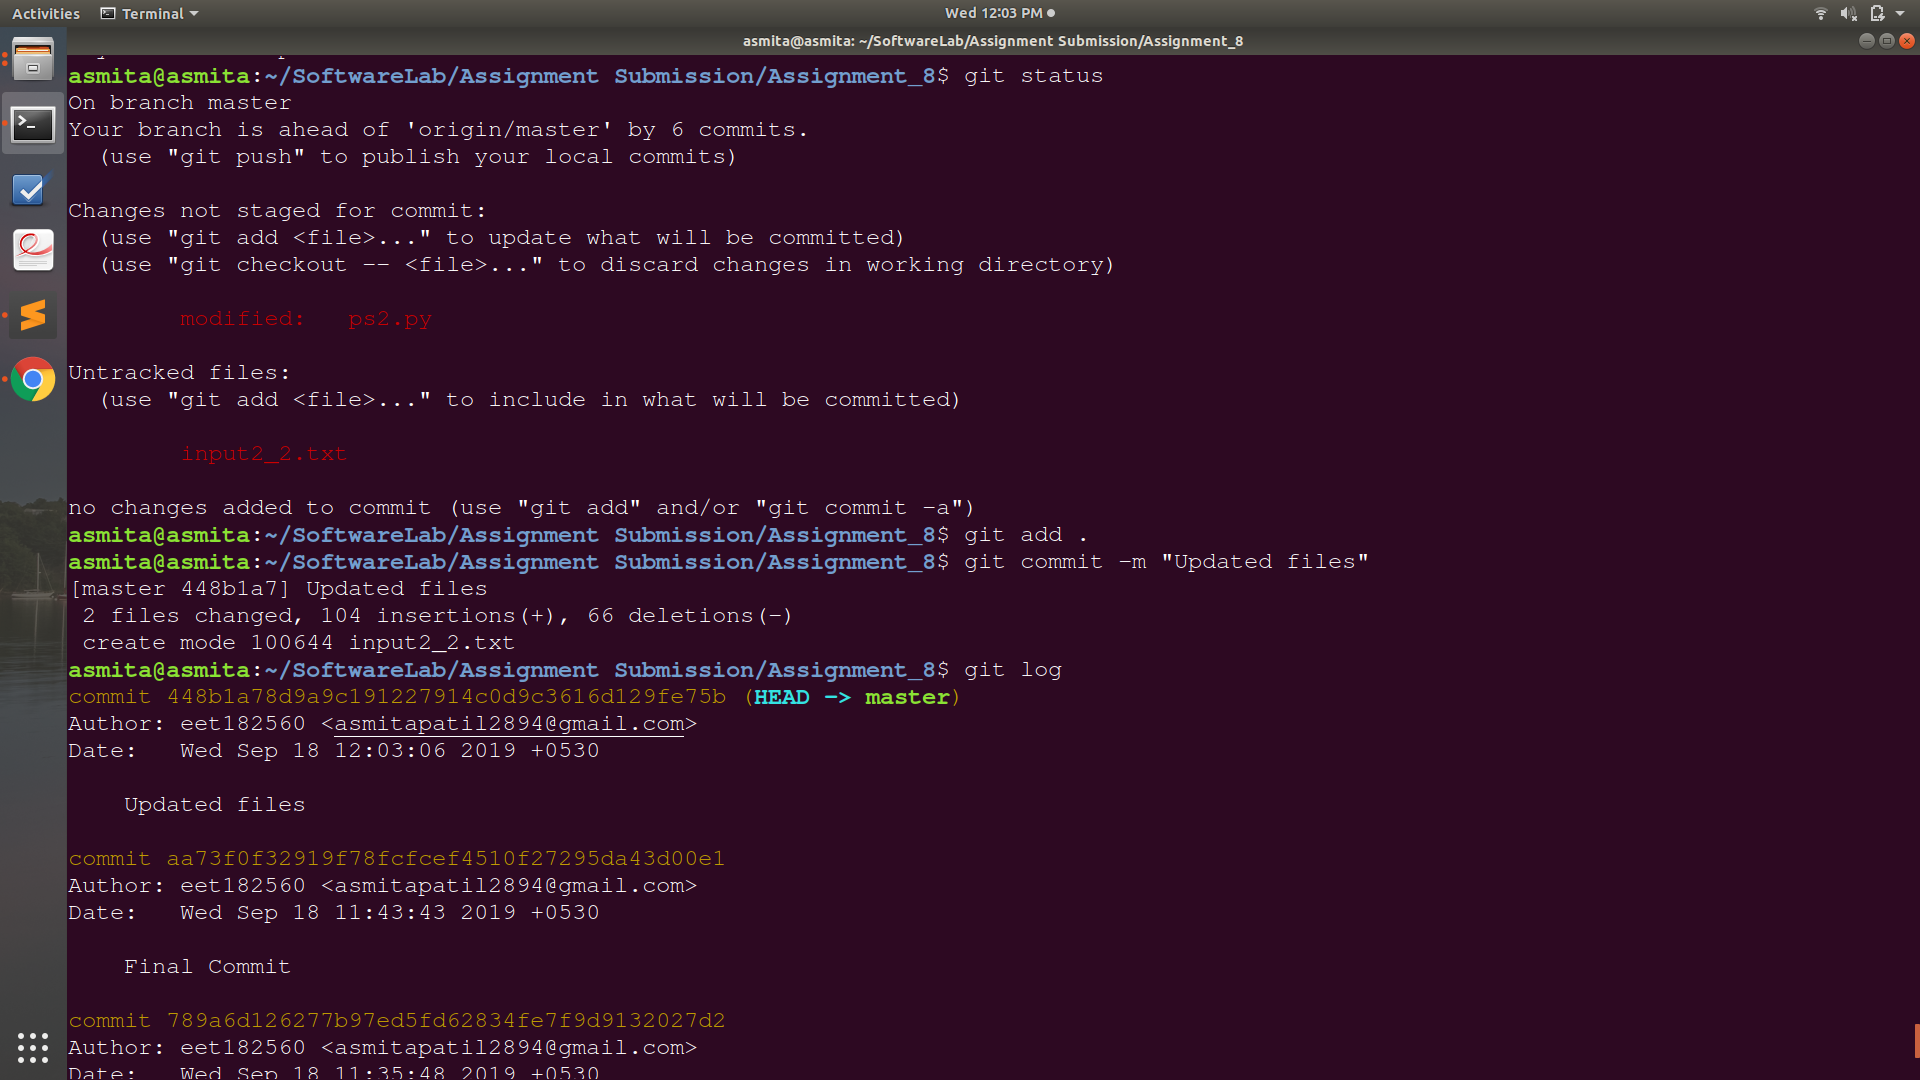
\includegraphics[width=1\textwidth]{Software_Lab_Template/images/git.png}
  \caption{Execution of Git Command}
  \label{fig:Execution of Git Command}
\end{figure}
\begin{figure}[h]
    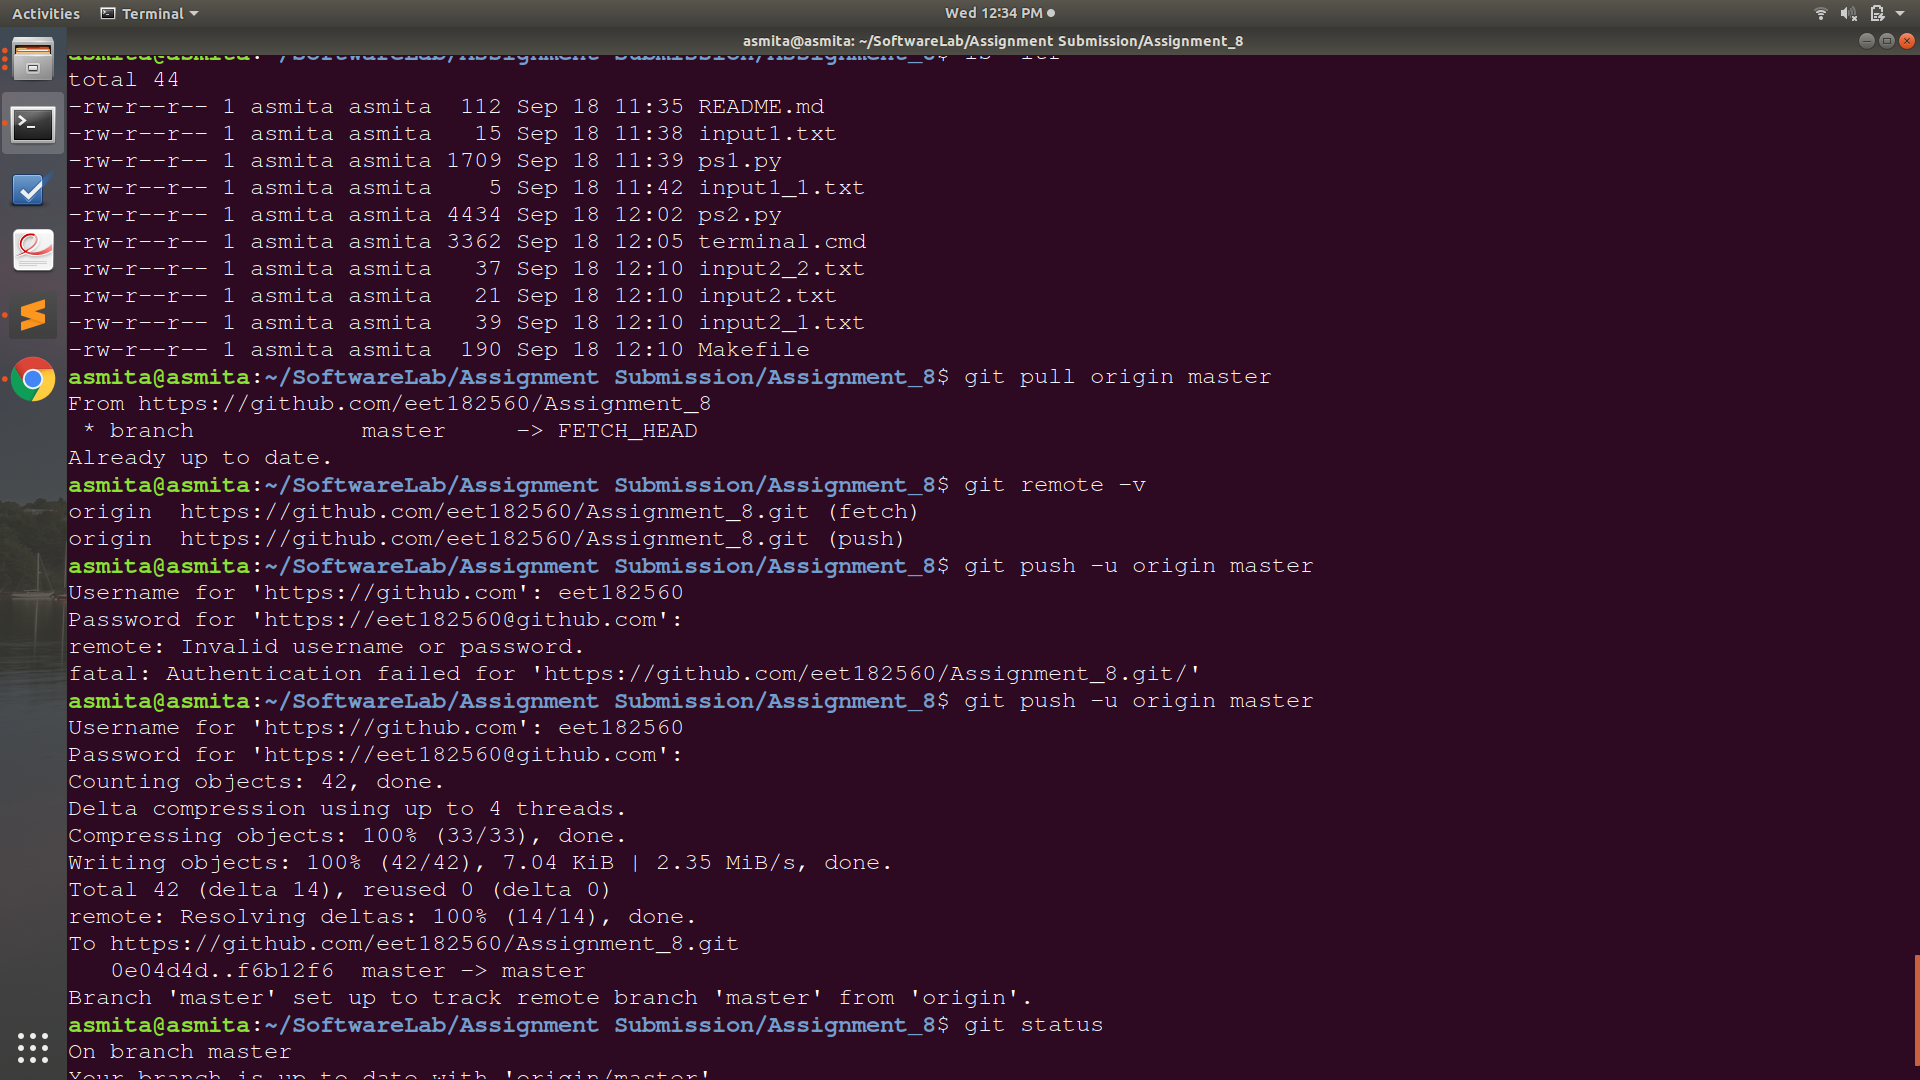
\includegraphics[width=1\textwidth]{Software_Lab_Template/images/1.png}
  \caption{Execution of Git Command}
  \label{fig:Execution of Git Command}
\end{figure}

\chapter{\textbf{Problem Statement-2}}
\section{Problem Statement}
\begin{itemize}
    \item \textbf{3X3 Numeric Tic-Tac-Toe (Use numbers 1 to 9 instead of X’s and O’s)}
    \item One player plays with the odd numbers (1, 3, 5, 7, 9) and the other player plays with the even numbers (2,4,6,8). All numbers can be used only once. 
    \item The player who puts down 15 points in a line wins (sum of 3 numbers). 
    \item Always Player with odd numbers starts the game. 
    \item Once a line contains two numbers whose sum is 15 or greater, there is no way to complete that line, although filling in the remaining cells might be necessary to complete a different line.
    \item Note – Line can be horizontal, vertical or diagonal

\end{itemize}

\section{Assumptions}
\begin{itemize}
    \item All basics commands of GIT are known to user and user have some hands on experience with GIT
    \item Basics concepts of String and list in python are known to user.
\end{itemize}

\section{Program Structure}

% Define block styles
\tikzstyle{decision} = [diamond, draw, fill=red!30, 
    text width=4.5em, text badly centered, node distance=2.5cm, inner sep=0pt]
\tikzstyle{block} = [rectangle, draw, fill=blue!30, 
    text width=10em, text centered, rounded corners, minimum height=4em]
\tikzstyle{line} = [draw, -latex']
\tikzstyle{cloud} = [draw, ellipse,fill=red!20, node distance=3cm,
    minimum height=2em]
    
\begin{tikzpicture}[node distance = 2cm, auto]
    % Place nodes
    \node [block] (init) {Start a Game};
    \node [block, below of=init] (identify) {Take input from player for pos & number};
    \node [decision, below of=identify] (decide1) {Are inputs valid?};
    \node [block, below of=decide1, node distance=2.5cm] (evaluate) {Display current Game Status to user};
    \node [decision, below of=evaluate] (decide2) {Is anyone winning or Draw?};
    \node [block, below of=decide2, node distance=2.5cm] (evaluate1){Ask user to continue or exit};
    \node [decision, below of=evaluate1] (decide3) {Exit?};
    \node [block, below of=decide3, node distance=2cm] (stop) {stop};
   
    % Draw edges
    \path [line] (init) -- (identify);
    \path [line] (identify) -- (decide1);
    \path [line] (decide1) -- node {yes} (evaluate);
    \path [line] (evaluate) -- (decide2);
    \path [line] (decide2) --  node {yes} (evaluate1);
    \path [line] (evaluate1) -- (decide3);
    \path [line] (decide3) -- (stop);
    \path [line] (decide1.west) to[out=180,in=150] (identify.west);
    \path [line] (decide2.west) to[out=180,in=150] (identify.west);
    \path [line] (decide3.west) to[out=180,in=150] (init.west);
\end{tikzpicture}

\section{Algorithm and Implementation}
Problem can be solved when execution is done in following steps:
\textit{
\begin{itemize}
    \item Take input from Player for position and number.
    \item Check validity of position and number for given constraints and current player.
    \item Display current board status/ Game Status to user.
    \item Check for winner if exists then ask user to exit the game or continue with new game.
    \item Winning condition will be checked across rows, columns and diagonally.
    \item Switch the player and go to step 1.
    \item Handle boundary conditions and flag error appropriately.
    \item Display required output when required.
\end{itemize}
Implementation is done in Python and screenshot, code snippet is attached for the same.
}

\section{Input and Output format}
\begin{itemize}
    \item \textbf{Input : }
        \begin{itemize}
            \item Get the position and number to be entered from the user.
            \item Get input from user in case of draw or any of the two players is winner to continue with new game or to exit

        \end{itemize}
    \item \textbf{Output : }
        \begin{itemize}
            \item Print ‘Welcome to the Game!’.	
            \item Print whether it is Player 1’s or Player 2’s chance.
            \item Show tic tac toe with data.
            \item \textbf{Sample output}:\\
            Welcome to the Game!\\
            Player 1’s chance\\
            Enter the position and number to be entered: 5,3\\
        \end{itemize}
    \item \textbf{Constraint :}
        \begin{itemize}
            \item 1$<=$Position$<=$9
            \item 1$<=$Number$<=$9
        \end{itemize}
        
\end{itemize}

\section{Test cases}
Following test cases are executed :
\begin{itemize}
    \item Input which gives normal output is executed
    \item Input which results into error is executed\\
Screenshots of output are shown below.
\end{itemize}

\section{Difficulties/Issues faced}
\begin{itemize}
    \item Difficult to find position to calculate sum row wise, column wise and diagonally. Solved using pre-defined arrays.
\end{itemize}

\section{Screenshots}
Following are the screenshots
\begin{figure}[h]
    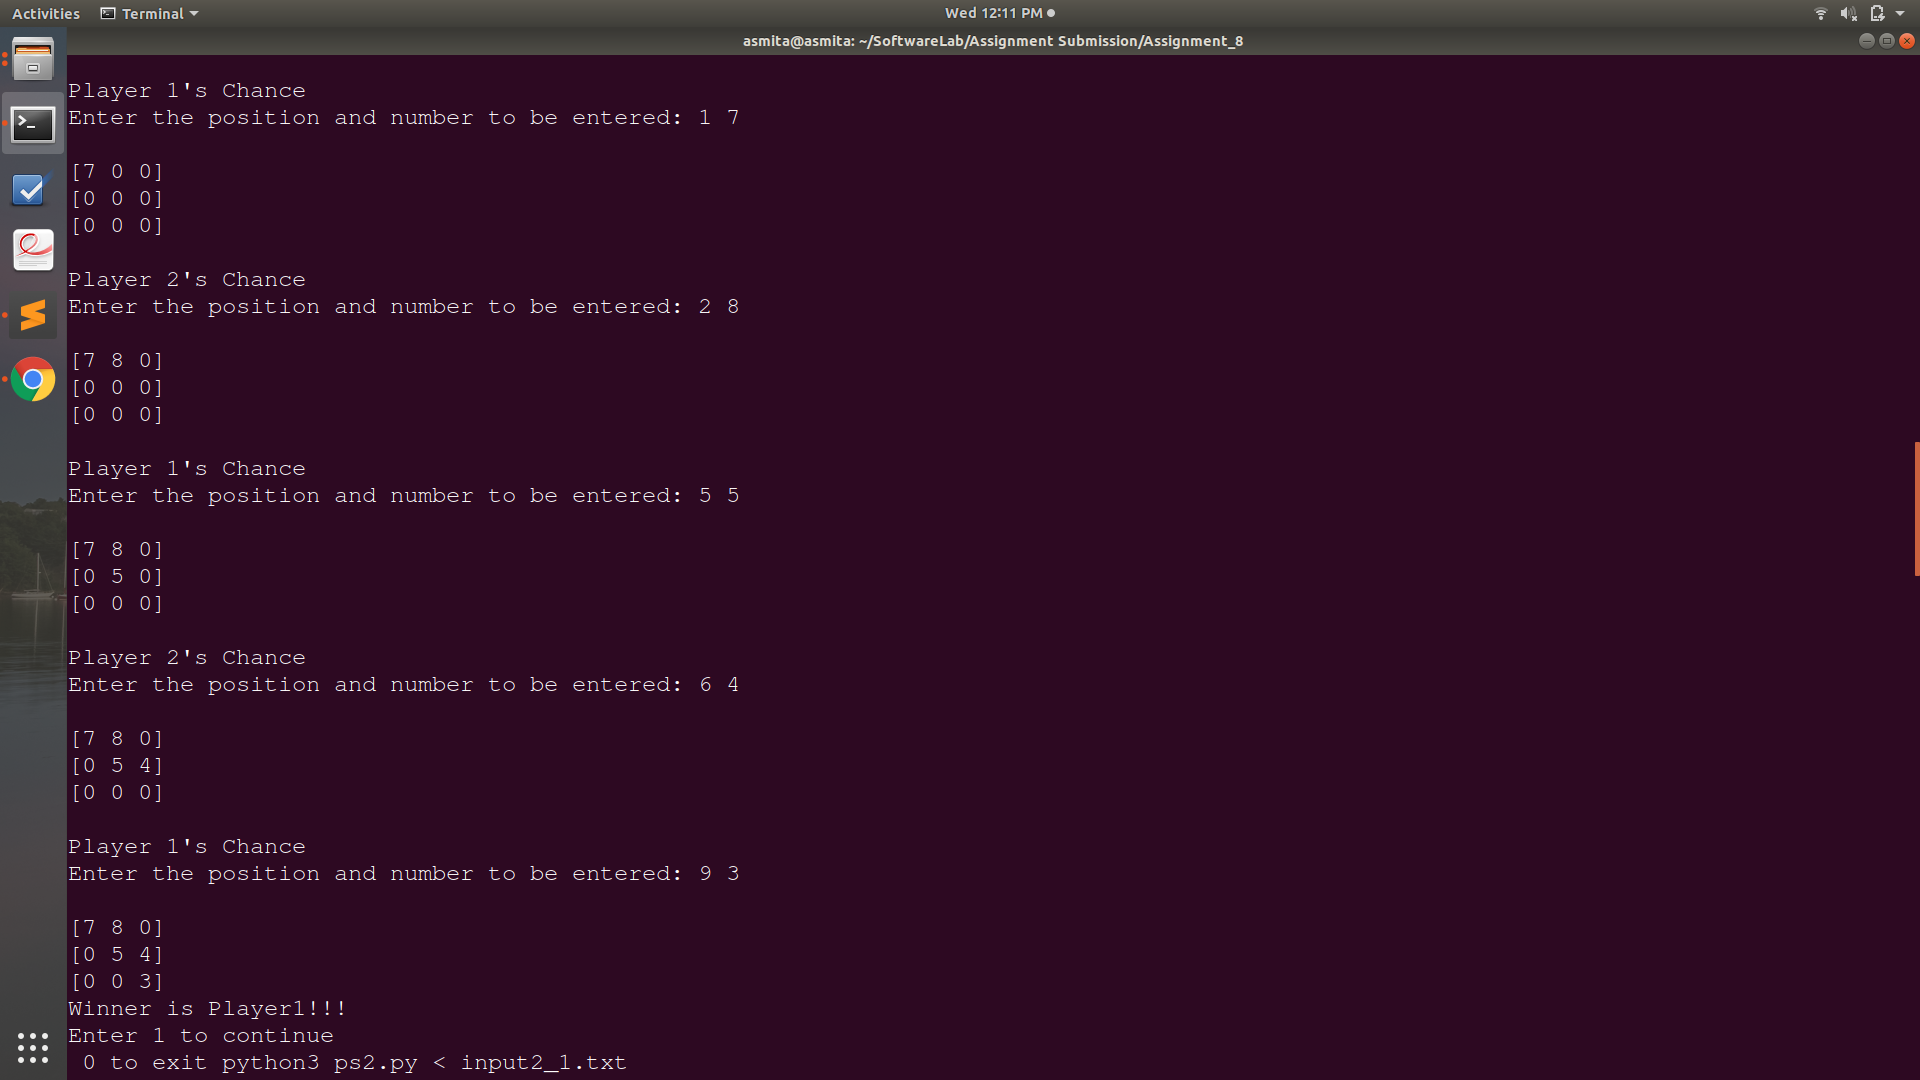
\includegraphics[width=1\textwidth]{Software_Lab_Template/images/normalExitPS2.png}
  \caption{Execution of problem statement 2: Normal Exit}
  \label{fig:Problem statement 2}
\end{figure}
\begin{figure}[h]
    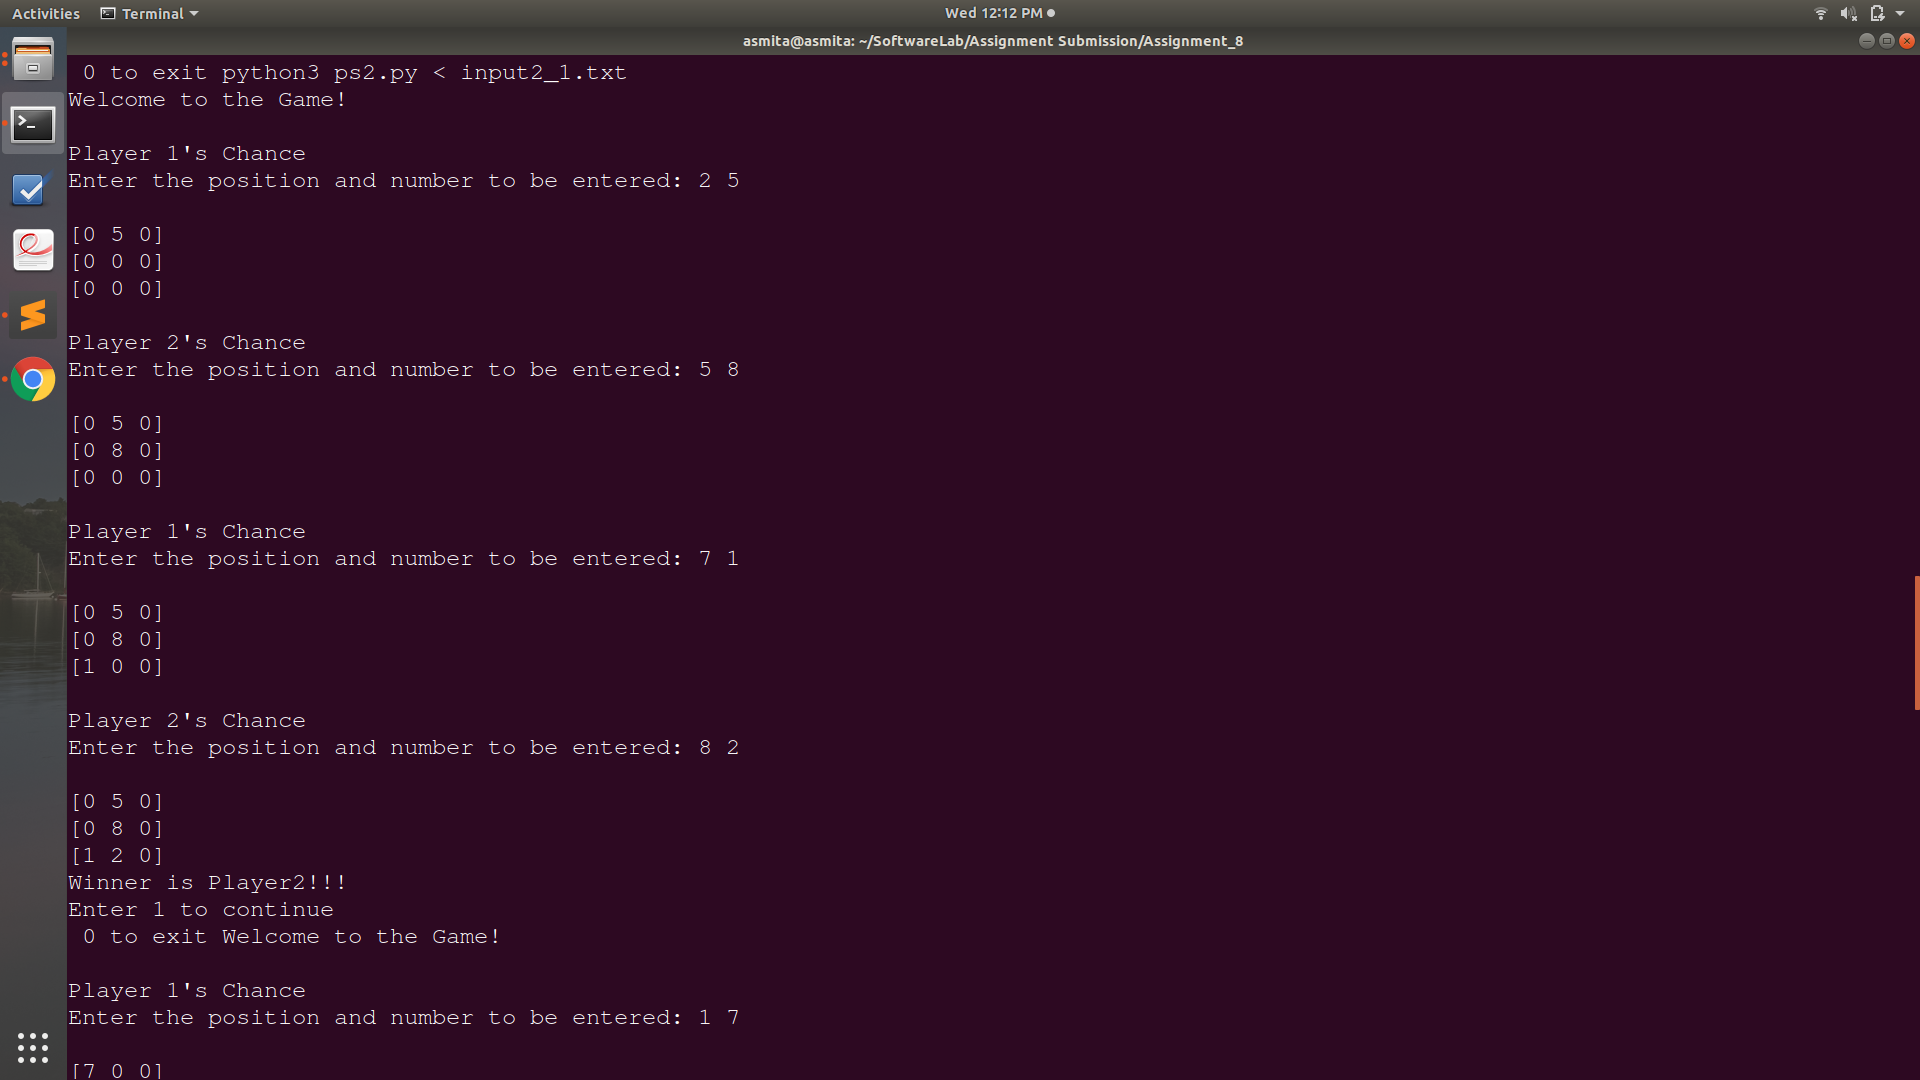
\includegraphics[width=1\textwidth]{Software_Lab_Template/images/ContinuePS2.png}
  \caption{Execution of problem statement 2: Continue with new Game}
  \label{fig:Problem statement 2}
\end{figure}
\begin{figure}[h]
    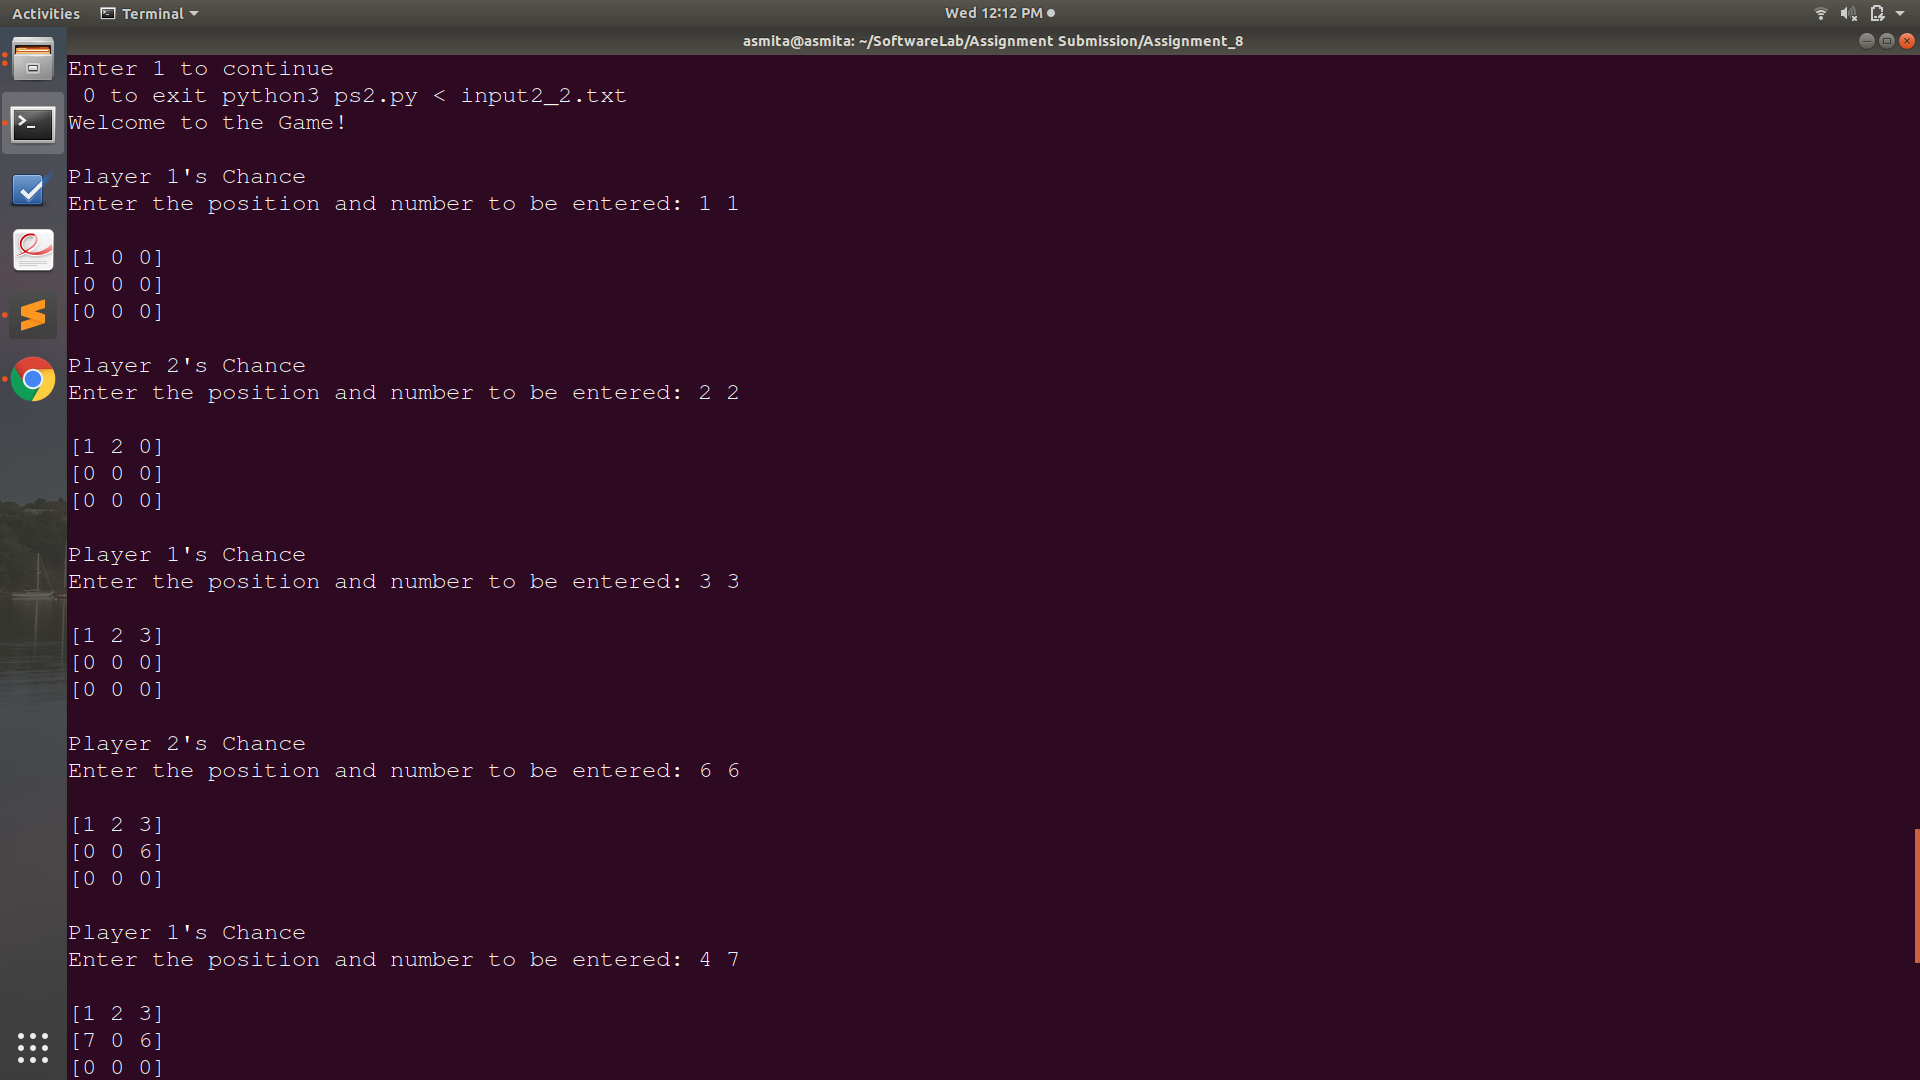
\includegraphics[width=1\textwidth]{Software_Lab_Template/images/DrawCase1.png}
  \caption{Execution of problem statement 2: Draw Case1}
  \label{fig:Problem statement 2}
\end{figure}
\begin{figure}[h]
    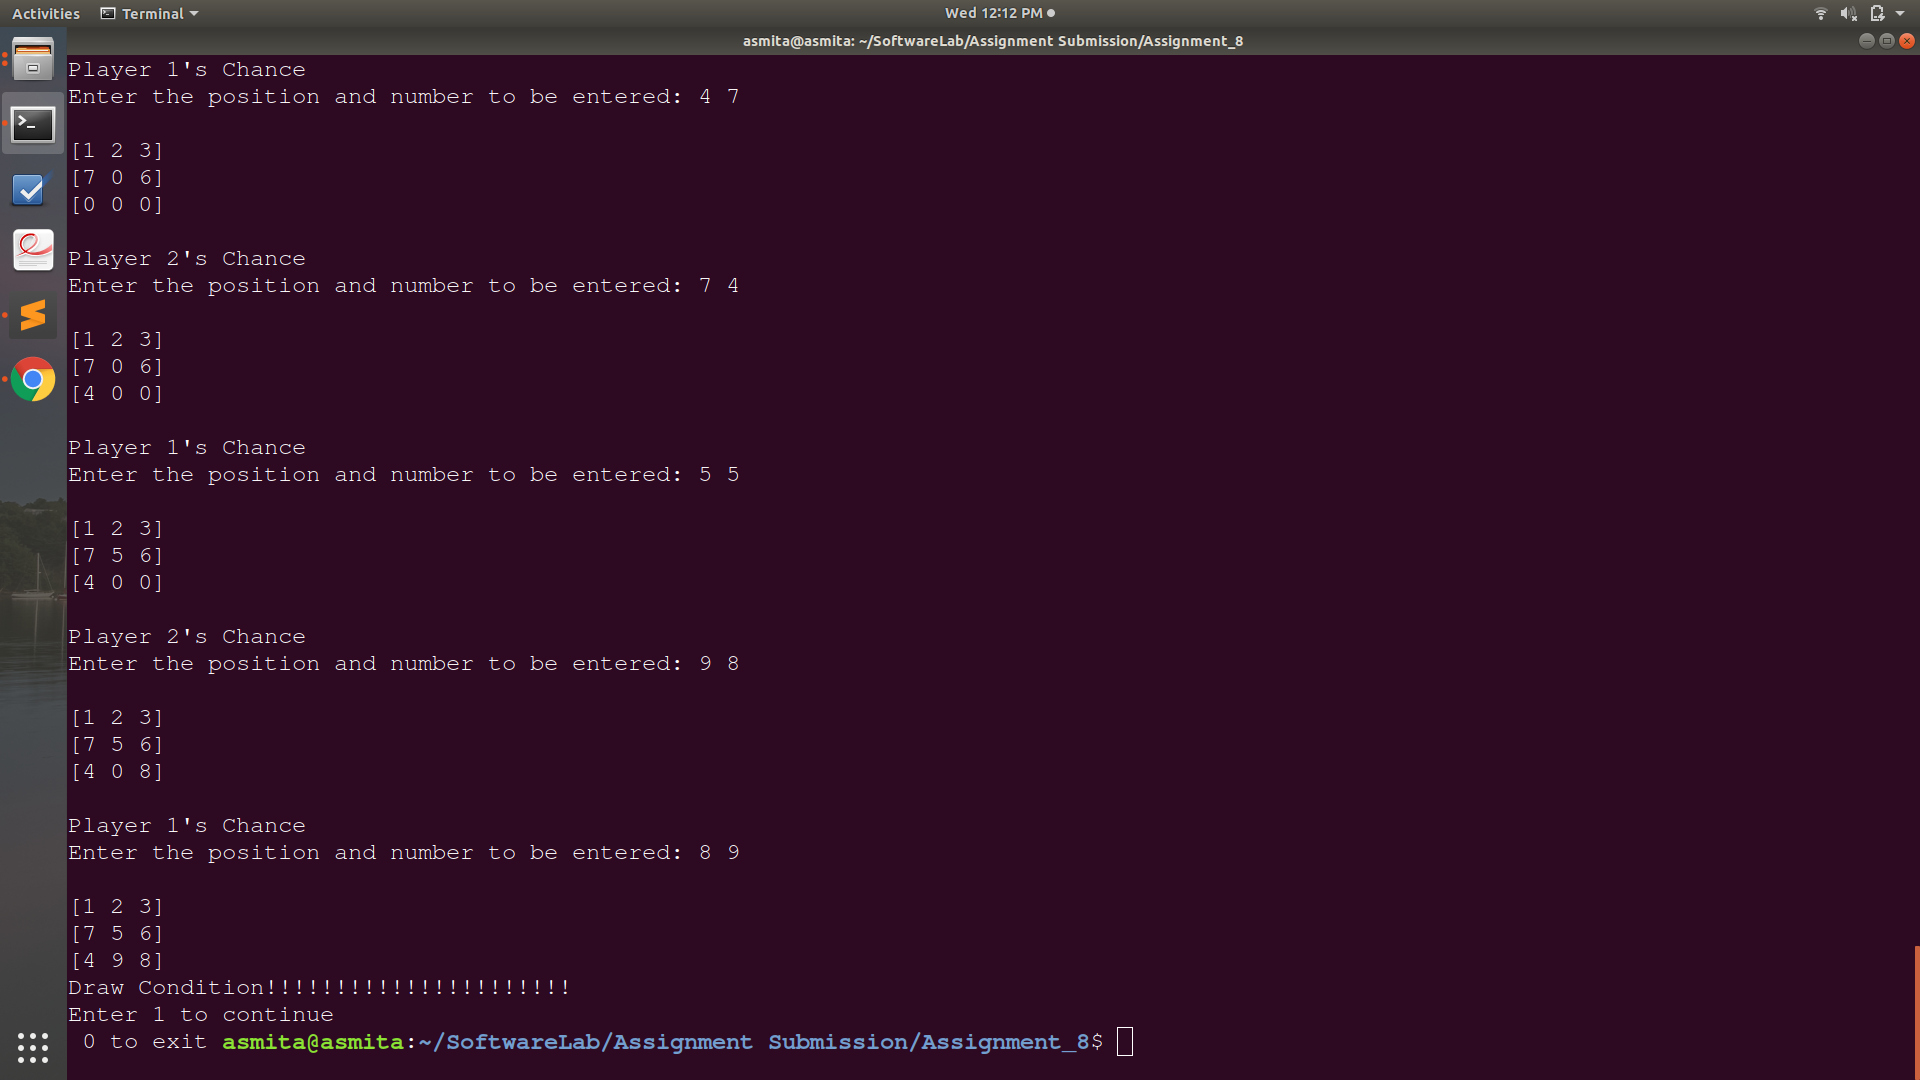
\includegraphics[width=1\textwidth]{Software_Lab_Template/images/DrawCase2.png}
  \caption{Execution of problem statement 2: Draw case2}
  \label{fig:Problem statement 2}
\end{figure}

%Appendix
\begin{appendices}
\chapter{Code for Problem Statement 1}

\begin{lstlisting}[language=Python, frame='single']
# Function Defintions
# Function which check validity of string if it is binary or not
def checkVal(String):
	# Convert string into list
	newList = list(String)
	# Check string character by character 
	for char in newList:
		if char == '0' or char == '1':
			continue
		else:
			return -1;

	# Return 0 if in case of valid string else -1
	return 0;


# Function to calculate parity of string
def calcParity(String):

	# Initialization of variables
	i = 0
	count = 0

	# Count numbers of 1's
	while i < len(String):
		if String[i] == '1':
			count += 1
		i += 1

	# Check number of 1's is odd or even
	if count % 2 == 0:
		count = 1
	else:
		count = 0

	# Return parity
	return count


# Function which generate transmission data after bit stuffing if required
def generateTransmissiondata(strParity):

	# Initialization of variables
	i = 0
	j = 0

	# Copying string into list to append
	newStr = list(strParity)

	# Check for pattern '010' in input data
	while i < len(strParity) - 3:

		# If pattern is found append it with 0
		if strParity[i : i + 3] == '010':
			newStr.insert(j + 3, '0')
			i += 2
			j += 3
		i += 1
		j += 1

	# Return string with flag appended '0101' 
	return ''.join(newStr) + '0101'

## Execution start from here
# Take input from user
String = input("Enter the binary String :")
print(String)
#Check validity of String
if checkVal(String) == -1:
	print("Invalid input")
	exit(0)

# Calculate parity of string and print the string with parity
count = calcParity(String)
strParity = String + str(count)
print("Parity bit data : " + strParity)

# Calculate data to be transmitted and print the same
outPut = generateTransmissiondata(strParity)
print("Transmitting data: " + outPut)



\end{lstlisting}

\chapter{Code for Problem Statement 2}
\begin{lstlisting}[language=Python, frame='single']
import numpy as np

# Function Declarations and Definitions
# Display the matrix / board
def display(mat):
	print()
	print(mat[0: 3])
	print(mat[3 : 6])
	print(mat[6 : 9])


# Function to check sum is 15 or not and exit based on it
def sumCheck(sum, player):
	if sum == 15:		
		print("Winner is Player" + str(player) + "!!!")
		flag = input("Enter 1 to continue\n 0 to exit ")
		if flag == "1":
			Game()
		else:
			exit(0)


# Function to calculate sum rowwise based on pos
def rowSum(mat, pos, player, vis):

	#Initialization of variables
	sum = 0
	valid = False

	# Calculate sum for first row pos
	if pos in row1:
		sum = mat[0] + mat[1] + mat[2]
		if vis[0] and vis[1] and vis[2]:
			valid = True

	# Calculate sum for second row pos
	elif pos in row2:
		sum = mat[3] + mat[4] + mat[5]
		if vis[3] and vis[4] and vis[5]:
			valid = True

	# Calculate sum for third row pos
	else:
		sum = mat[6] + mat[7] + mat[8]
		if vis[6] and vis[7] and vis[8]:
			valid = True

	# Check validity of the sum and call sumCheck
	if valid:
		sumCheck(sum, player)


# Function to calculate sum column wise based on pos
def colSum(mat, pos, player, vis):

	#Initialization of variables
	sum = 0
	valid = False

	# Calculate sum for first column position
	if pos in col1:
		sum = mat[0] + mat[3] + mat[6]
		if vis[0] and vis[3] and vis[6]:
			valid = True

	# Calculate sum for second column position
	elif pos in col2:
		sum = mat[1] + mat[4] + mat[7]
		if vis[1] and vis[4] and vis[7]:
			valid = True

	# Calculate sum for third column position
	else:
		sum = mat[2] + mat[5] + mat[8]
		if vis[2] and vis[5] and vis[8]:
			valid = True

	# Check validity of the sum and call sumCheck
	if valid:
		sumCheck(sum, player)

# Function to calculate sum diagonally based on pos
def diagonal(mat, pos, player, vis):

	#Initialization of variables
	sum = 0
	valid = False

	# Calculate sum for second diagonal position
	if pos in diagonal1:
		sum = mat[0] + mat[4] + mat[8]
		if vis[0] and vis[4] and vis[8]:
			valid = True

	# Check validity of the sum and call sumCheck
	if valid:
		sumCheck(sum, player)

	# Calculate sum for second diagonal position
	if pos in diagonal2:
		sum = mat[2] + mat[4] + mat[6]
		if vis[2] and vis[4] and vis[6]:
			valid = True

	# Check validity of the sum and call sumCheck
	if valid:
		sumCheck(sum, player)


#Check for draw condition
def checkDraw(vis):
	flag = True
	for i in vis:
		if i == False:
			flag = False
			break

	# if draw then give user option to continue or exit
	if flag:
		print("Draw Condition!!!!!!!!!!!!!!!!!!!!!!")
		flag = input("Enter 1 to continue\n 0 to exit ")
		if flag == "1":
			Game()
		else:
			exit(0)


# Function to start a game
def Game():

	# Initialization of all variables
	mat = np.zeros(9, dtype=np.int32)
	vis = [False] * 9
	numVis = [False] * 9
	
	# Start of game with player1
	print("Welcome to the Game!")
	player = 1

	# Infinite to execute game
	while True:

		# take user input for position and number to be used
		print()
		print("Player " + str(player) + "'s Chance")
		pos, num = input("Enter the position and number to be entered: ").split(",")
		print(pos, num)

		# Check validity of position
		pos = int(pos)
		if pos < 1 or pos > 9:
			print("Invalid position")
			continue

		# Check validity of number
		num = int(num)
		if num < 1 or num > 9:
			print("Invalid number")
			continue

		# Check validity of number based on player's chance
		if player == 1 and num not in player1:
			print("Please enter odd number")
			continue
		elif player == 2 and num not in player2:
			print("Please enter even number")
			continue

		# Check validity of number and position 
		if vis[pos - 1] == True:
			print("Enter the position which is not used")
			continue
		if numVis[num - 1] == True:
			print("Enter the number which is not used yet")
			continue

		# update the variables for given input
		vis[pos - 1] = True
		numVis[num - 1] = True 
		mat[pos - 1] = num

		# Display current board status
		display(mat)

		# Check for winner if exists end the game else continue
		rowSum(mat, pos, player, vis)
		colSum(mat, pos, player, vis)
		diagonal(mat, pos, player, vis)	

		checkDraw(vis)

		# Switch the player
		if player == 1:
			player = 2
		else:
			player = 1


### Execution starts from here

player1 = {1, 3, 5, 7, 9}
player2 = {2, 4, 6, 8}
row1 = {1, 2, 3}
row2 = {4, 5, 6}
col1 = {1, 4, 7}
col2 = {2, 5, 8}
diagonal1 = {1, 5, 9}
diagonal2 = {3, 5, 7}
Game()

\end{lstlisting}

\chapter{Code for Makefile}

\begin{lstlisting}[language=make, frame='single']
all: ps1 ps2

ps1: ps1.py
	python3 ps1.py < input1.txt
	python3 ps1.py < input1_1.txt

ps2: ps2.py
	python3 ps2.py < input2.txt
	python3 ps2.py < input2_1.txt
	python3 ps2.py < input2_2.txt

\end{lstlisting}


\chapter{Output of history command from terminal}
\verbatiminput{terminal.cmd}

\end{appendices}

\printbibliography


\end{document}
